\section{Background and Related Work}
\label{sec:background}

We describe %OIDC \cite{OpenIDConnect}, to describe
typical SSO services and discuss existing privacy-preserving solutions and other related works.

\subsection{OpenID Connect and SSO Services}
\label{subsec:OIDC}
OIDC is one of the most popular SSO protocols. It supports different login flows: implicit flow, authorization code flow, and hybrid flow (a mix of the other two). These flows differ in the steps for requesting and receiving identity tokens but have common security requirements for identity tokens. We present our designs in the implicit flow and discuss the support for the authorization code flow in Section \ref{sec:discussion}.

In OIDC, users and RPs register at an IdP with their identities
and other information such as user credentials %(e.g., passwords)
and RP endpoints. %(i.e., the URLs to receive tokens).
As shown in Figure \ref{fig:OpenID}, when an RP receives a login request, it constructs an identity-token request with its own identity and the scope of requested user attributes.
This request is redirected to the IdP. Once the IdP authenticates the user, it issues an identity token that encloses the identities (or pseudo-identities) of the user and the visited RP, the requested user attributes, a validity period, etc. The user then forwards the identity token to the RP's endpoint. The RP verifies the token and allows the holder to log in as the enclosed (pseudo-)identity.

% The user's operations, e.g., request redirection, authorization, and token forwarding, are performed by user agents, such as a browser for web applications.
% 这个浏览器相关的词句,放到后面的实现章节。

\begin{figure}[t]
  \centering
  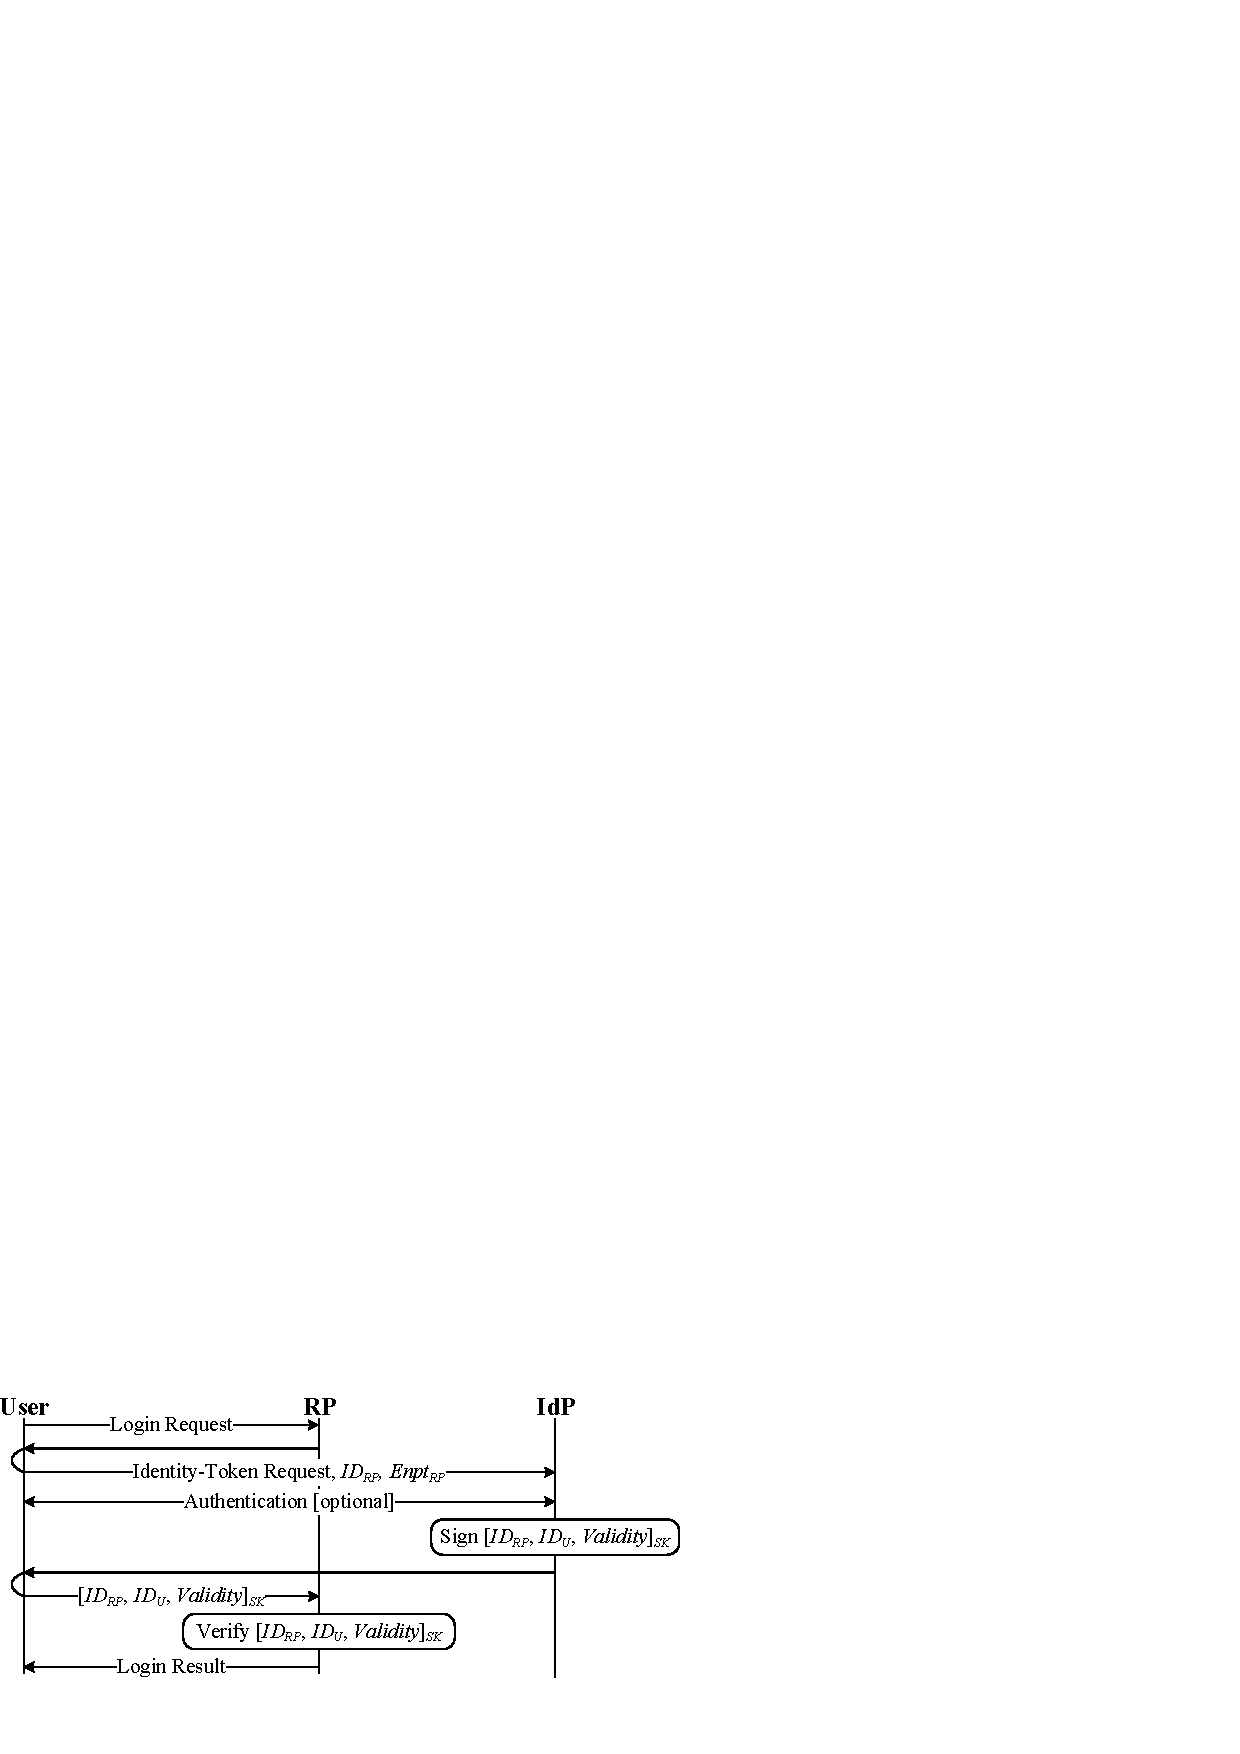
\includegraphics[width=0.95\linewidth]{fig/OIDC.pdf}
  \caption{The implicit SSO login flow of OIDC}
  \label{fig:OpenID}
\end{figure}

\begin{table*}[tb]
\footnotesize
    \caption{Privacy-preserving solutions for SSO and identity federation}
    \centering
    \begin{tabular}{|c|c|c|c|c|c|c|}
  \hline
  \multirow{3}*{\textbf{~~Solution~~}} &
  \multicolumn{3}{c|}{\textbf{SSO Feature} - supported $\CIRCLE$, unsupported $\Circle$, or partially $\LEFTcircle$} & \multicolumn{3}{c|}{\textbf{Privacy Threat} - prevented $\CIRCLE$ or not $\Circle$} \\ \cline{2-7}
  & User Identification & User Authentication & IdP-confirmed Selective  & IdP-based & RP-based & Server \\
  & at each RP & only to the IdP &  Attribute Provision & Login Tracing & Identity Linkage & Collusion$^{\dag}$ \\\hline
  OIDC w/ PPID \cite{NIST2017draft} & $\CIRCLE$ & $\CIRCLE$ & $\CIRCLE$ & $\Circle$ & $\CIRCLE$ & $\Circle$ \\ \hline
  MISO \cite{miso} & $\CIRCLE$ & $\CIRCLE$ & $\CIRCLE$ & $\CIRCLE$ & $\CIRCLE$ & $\Circle$$^1$  \\ \hline 
  BrowserID \cite{BrowserID} & $\CIRCLE$ & $\CIRCLE$$^2$ & $\Circle$ & $\CIRCLE$ & $\Circle$ & $\Circle$ \\ \hline
  SPRESSO \cite{SPRESSO} & $\CIRCLE$ & $\CIRCLE$ & $\LEFTcircle$$^3$ & $\CIRCLE$ & $\Circle$ & $\Circle$ \\ \hline
  PRIMA \cite{prima} & $\CIRCLE$ & $\Circle$ & $\CIRCLE$ & $\CIRCLE$ & $\Circle$ & $\Circle$ \\ \hline
  PseudoID \cite{PseudoID} & $\CIRCLE$ & $\Circle$ & $\LEFTcircle$$^4$ & $\CIRCLE$ & $\CIRCLE$ & $\CIRCLE$ \\ \hline
  Opaak \cite{Opaak} & $\LEFTcircle$$^5$ & $\Circle$ & $\Circle$ & $\CIRCLE$ & $\CIRCLE$ & $\CIRCLE$ \\ \hline
 % U-Prove \cite{uprov} & $\CIRCLE$ & $\Circle$ & $\LEFTcircle$$^6$ & $\CIRCLE$ & $\CIRCLE$ & $\CIRCLE$ \\ \hline
 % UnlimitID \cite{UnlimitID} & $\CIRCLE$ & $\Circle$ & $\CIRCLE$ & $\CIRCLE$ & $\CIRCLE$ & $\CIRCLE$ \\ \hline
 % EL PASSO \cite{ELPASSO} & $\CIRCLE$ & $\Circle$ & $\CIRCLE$ & $\CIRCLE$ & $\CIRCLE$ & $\CIRCLE$ \\ \hline
  \cite{ELPASSO,uprov,UnlimitID} & $\CIRCLE$ & $\Circle$ & $\CIRCLE$$^6$ & $\CIRCLE$ & $\CIRCLE$ & $\CIRCLE$ \\ \hline
  Fabric Idemix \cite{hyperledge-idemix} & $\LEFTcircle$$^7$ & $\Circle$ & $\CIRCLE$ & $\CIRCLE$ & $\CIRCLE$ & $\CIRCLE$ \\ \hline
 % PrivacyPass \cite{privacypass,trusttoken} & $\Circle$ & $\Circle$ & $\Circle$ & $\CIRCLE$ & $\CIRCLE$ & $\Circle$ \\ \hline
  \usso & $\CIRCLE$ & $\CIRCLE$ & $\CIRCLE$ & $\CIRCLE$ & $\CIRCLE$ & $\Circle$ \\ \hline
\end{tabular}
    \label{tbl:comparison-protocol}
\flushleft
{\footnotesize
$^{\dag}$. This threat happens when \emph{all} servers involved in the processing of identity tokens collude.\\
1. MISO is immune to collusive attacks by the IdP and RPs, but another \emph{fully-trusted} server called mixer is involved in the identity-token generation.\\
2. A BrowserID user generates an \emph{ephemeral} private key to sign subsidiary ``identity assertion'' tokens,
also verified by the RP.\\
3. SPRESSO can be extended to provide selective user attributes in the tokens, while the prototype does not implement this feature.\\
4. Blindly-signed user attributes can be selectively provided using zero-knowledge proofs but not implemented in the prototype.\\
5. Opaak supports two exclusive pseudonym options: (\emph{a}) linkable within an RP but unlinkable across multiple RPs and (\emph{b}) unlinkable for any pair of actions.\\
6. Different from \cite{ELPASSO,UnlimitID}, a credential in U-Prove \cite{uprov} may contain some attributes that are \emph{invisible} to the IdP, in addition to the ones confirmed by the IdP.\\
7. In the original design of Idemix \cite{idemix}, every user logs into an RP with a unique account, but Fabric Idemix implements completely-anonymous services.}
\end{table*}

The following features are desired in SSO services and supported by popular SSO systems \cite{NIST2017draft, OpenIDConnect,rfc6749, SAML, SAMLIdentifier}.

\noindent \textbf{Unique user identification at an RP.}
An RP recognizes each user by a \emph{unique} identity (or account) at the RP to provide customized services across multiple logins.
Such a non-anonymous SSO system is much more desirable in various scenarios than anonymous services.

\noindent\textbf{User authentication only to the IdP.}
RPs only verify the identity tokens issued by an IdP, and the authentication between a user and the IdP is typically conducted \emph{independently} of the steps that deal with identity tokens.
This offers advantages. First, the IdP authenticates users by any appropriate means such as passwords, one-time passwords, or multi-factor authentication.
Meanwhile, a user only maintains her credential at the IdP; and if it is lost or leaked, the user only needs to renew it at the IdP.
However, if a user proves a \emph{non-ephemeral} secret to RPs that is valid across multiple logins, she will have to notify each RP in the events of loss or leakage, or additional revocation checking will be needed \cite{ELPASSO, UnlimitID}.

\noindent\textbf{Selective IdP-confirmed attribute provision.}
An IdP usually includes user attributes in identity tokens \cite{OpenIDConnect,rfc6749} along with user (pseudo-)identities.
A user maintains these attributes at the trusted IdP,
which obtains the user's authorization before enclosing attributes or provides only pre-selected attributes.

\subsection{Privacy-Preserving SSO and Identity Federation}
\label{subsec-solutions}

Privacy-preserving SSO is expected to offer the desired features listed in Section \ref{subsec:OIDC} while addressing different privacy threats.
In contrast, privacy-preserving identity federation offers more privacy protections but introduces extra complexity in the user authentication process.
Identity federation enables a user registered at a trusted IdP to be accepted by other parties, potentially with different accounts,
but \emph{additional user operations for the authentication steps between the user and RPs} are involved.\footnote{SSO protocols \cite{OpenIDConnect,rfc6749, SAML, SAMLIdentifier} allow a user to log into an RP \emph{without} maintaining an account at the RP by herself or holding a permanent secret to be verified by the RP. Although the same term ``single sign-on (SSO)'' was used in other schemes \cite{PseudoID, Opaak, ELPASSO, WangWS13, HanCSTW18, HanCSTWW20}, they are different from the widely-used SSO protocols because a user needs to maintain the accounts at different RPs and/or hold a permanent secret verified by the RPs. In this paper, we refer to them as \emph{identity federation} to emphasize this difference.}
As shown in Table \ref{tbl:comparison-protocol}, none of the existing solutions 
perfectly satisfies all expectations.


\noindent\textbf{Privacy-preserving SSO.}
Existing privacy-preserving SSO approaches \cite{BrowserID, SPRESSO, NIST2017draft} prevent either IdP-based login tracing or RP-based identity linkage, but not both.
Pairwise pseudonymous identifiers (PPIDs) are specified \cite{OpenIDConnect, SAMLIdentifier} and recommended \cite{NIST2017draft}
for protecting user privacy against curious RPs.
An IdP creates a unique PPID for a user to log into some RP and encloses it in identity tokens, so colluding RPs cannot link the user.
It does not prevent IdP-based login tracing because the IdP needs the RP's identity to assign PPIDs.

MISO \cite{miso} decouples the calculation of PPIDs from an IdP,
        and another mixer server calculates a user's PPID
    based on $ID_U$, $ID_{RP}$ and a secret,
    after it receives the authenticated user's identity from the IdP.
MISO prevents both RP-based identity linkag, %for the RPs receives only PPIDs,
    and also IdP-based login tracing because $ID_{RP}$ is disclosed to the mixer but not the IdP.
It protects a user's online profile against even collusive attacks by the IdP and RPs,
    but it requires an extra fully-trusted mixer.
  %      which is ensured by Intel SGX.

% 这个就是扯淡吧?为什么还要网络通信呢?直接把Mixer实现在IdP内部,就行了吧?

Other privacy-preserving SSO schemes prevent IdP-based login tracing but leave users vulnerable to RP-based identity linkage, due to the unique user identities enclosed in identity tokens.
For example, in BrowserID \cite{BrowserID} %(formerly known as Firefox Accounts \cite{FirefoxAccount} and Mozilla Persona \cite{persona}),
the IdP %(called the primary identity authority in BrowserID)
issues a ``user certificate'' token that binds a user identity to an \emph{ephemeral} public key. The user then signs a subsidiary ``identity assertion'' token that binds the target RP's identity and sends both tokens to the RP. In SPRESSO \cite{SPRESSO} the RP creates a one-time pseudo-identity in each login, which is enclosed in identity tokens along with the user's unique identity.


\noindent\textbf{Privacy-preserving identity federation.}
In PRIMA \cite{prima}, the IdP signs a credential
that binds user attributes and a verification key. Using the signing key, the user selectively provides attributes to the RPs. This verification key works as the user's identity but exposes her to RP-based identity linkage.

%To protect user privacy against more threats, 
PseudoID \cite{PseudoID} introduces a service in addition to the IdP,
 to blindly sign \cite{blind-sign}
an access token that binds a pseudonym and a user secret.
The user then unblinds this token and uses the secret to log into an RP. Approaches based on anonymous credentials \cite{anon-credential-2001, idemix, anon-credential} have been proposed to implement privacy-preserving identity federation \cite{hyperledge-idemix, Opaak, uprov, UnlimitID, ELPASSO}. For instance, the IdP signs anonymous credentials in Opaak \cite{Opaak}, UnlimitID \cite{UnlimitID}, EL PASSO \cite{ELPASSO}, and U-Prove \cite{uprov}, and binds them with non-ephemeral user secrets. %, with which users can authenticate to an RP.
Then the users prove ownership of the anonymous credentials using the secrets and disclose IdP-confirmed attributes in the credentials in most schemes except Opaak.
Similarly, Hyperledger Fabric \cite{hyperledge-idemix} integrates Idemix anonymous credentials \cite{idemix} for completely-unlinkable pseudonyms and IdP-confirmed attribute disclosure.


These approaches \cite{PseudoID,Opaak,ELPASSO,uprov,UnlimitID,hyperledge-idemix} prevent both IdP-based tracing and RP-based identity linkage for (\emph{a}) the RP's identity is not enclosed in the anonymous credentials and (\emph{b}) the user selects different pseudonyms when visiting different RPs.
They even protect user privacy against collusive attacks by the IdP and RPs, as \emph{user-managed} pseudonyms cannot be linked through anonymous credentials \cite{anon-credential-2001, idemix, anon-credential} even when the ownership of these credentials is proved to RPs using one user secret.
However, this privacy protection results in additional user operations in identity federation, compared with widely-used SSO.
Users are required to maintain not only the authentication credentials for the IdP but also the long-term secrets that are verified by RPs.
For example, EL PASSO \cite{ELPASSO} requires users to keep the secrets securely on their devices and coordinate the credential revocation process \cite{ELPASSO, UnlimitID}.
Besides, the users locally manage their accounts at different RPs, and it actually involves authentication steps between the user and RPs, which is referred to as \emph{asynchronous authentication} \cite{ELPASSO}.


\noindent\textbf{Anonymous identity federation.}
Such approaches offer strong user privacy protections. They allow users to access RPs with pseudonyms that cannot be used to link any two access actions.
Anonymous identity federation was formalized \cite{WangWS13} and implemented using cryptographic primitives such as group signature and zero-knowledge proof \cite{WangWS13, HanCSTWW20, HanCSTW18}. Special features including proxy re-verification \cite{HanCSTWW20} and designated verification \cite{HanCSTW18}, are also supported. %in these schemes.
%and proposed for different applications such as GSM communications \cite{ElmuftiWRR08},
These completely-anonymous authentication services only work for special scenarios and do not support user identification at an RP, which is a common requirement in most applications.
